\documentclass[11pt,a4paper]{article}

\usepackage[utf8]{inputenc}
\usepackage[T1]{fontenc}
\usepackage{lmodern}
\usepackage[margin=1in]{geometry}
\usepackage{graphicx}
\usepackage{booktabs}
\usepackage{amsmath,amssymb}
\usepackage{microtype}
\usepackage{xcolor}
\usepackage[hidelinks]{hyperref}
\usepackage[round]{natbib}
\usepackage{caption}
\usepackage{float}

\captionsetup{font=small,labelfont=bf}
\newcommand{\todo}[1]{\textcolor{red}{[TODO: #1]}}

\title{Genome-level antibiotic resistance prediction in \textit{Escherichia coli}\\
from protein language model embeddings:\\
a comparison of set and sequence aggregation heads}

\author{
  Sachin \todo{surname}\\
  \textit{\todo{Affiliation}}\\
  \texttt{\todo{email}}
}
\date{\today}

\begin{document}
\maketitle

\begin{abstract}
Predicting whether a bacterial isolate resists an antibiotic from its genome could shorten the time to an effective treatment.
We study this problem on the BacBench antibiotic-resistance corpus, restricted to \textit{Escherichia coli}
(6{,}055 genomes with phenotype labels for 37 antibiotics).
Each genome contains roughly 4{,}700 distinct proteins, too many to encode end to end.
We therefore embed every unique protein once with a pretrained protein language model (ESM-2, 35M parameters),
de-duplicating 29.0 million protein occurrences to 1.35 million sequences, and train small heads that read all embeddings of a genome
and output resistance probabilities for every antibiotic simultaneously.
We compare five aggregation heads: mean pooling, gated attention-based multiple-instance learning, a Transformer encoder, a 1D CNN and a BiLSTM
(the last two read proteins in genome order).
On a held-out validation split of 605 genomes, the attention, CNN and Transformer heads reach a macro AUROC of 0.931, 0.925 and 0.923 over 21 antibiotics
with at least 10 resistant validation genomes, compared with 0.843 for mean pooling and 0.593 for an end-to-end baseline that sees 64 random proteins per genome.
The three best heads are indistinguishable given our single-seed evaluation.
We report these results as a preliminary benchmark: the split is random rather than lineage-aware, model selection used the same genomes as reporting,
and no gene presence/absence baseline is included.
We discuss these limitations and outline the experiments needed to turn the benchmark into firm conclusions.
\end{abstract}

\noindent\textbf{Keywords:} antimicrobial resistance, \textit{Escherichia coli}, protein language models, multiple-instance learning, genomics

\section{Introduction}
Antimicrobial resistance (AMR) is a growing clinical problem, and standard phenotypic susceptibility tests take a day or more after an isolate has been cultured.
Whole-genome sequencing is increasingly routine, which motivates models that predict a resistance phenotype directly from the genome.
Classical approaches look up known resistance genes and mutations, or train machine-learning models on gene presence/absence or $k$-mer features
\citep{moradigaravand2018}.
Protein language models such as ESM-2 \citep{lin2023} offer a different representation: a dense vector for each protein that captures properties learned from evolutionary-scale sequence data.

A bacterial genome is naturally a \emph{set} of proteins, and a resistance phenotype is often driven by a very small subset of them
(for example an enzyme that inactivates a drug or a mutated drug target) hidden among thousands of unrelated proteins.
This is the setting of multiple-instance learning \citep{ilse2018}: the label belongs to the bag (the genome), not to its instances (the proteins).
The practical difficulty is scale. A typical \textit{E.~coli} genome has about 4{,}700 distinct proteins, and encoding all of them with a protein model for every training step is expensive.

\paragraph{Contributions.}
\begin{enumerate}
  \item We define a genome-level, multi-antibiotic prediction task on the \textit{E.~coli} subset of the BacBench antibiotic-resistance corpus, with masked training for incompletely tested antibiotics.
  \item We show that de-duplicating proteins across genomes (a $\approx 21\times$ reduction) makes it feasible to embed every protein once and train on all of a genome's proteins on a single 22\,GB GPU.
  \item We compare five aggregation heads on identical embeddings, labels and split, and report per-antibiotic results.
  \item We state plainly what the current evidence does and does not support, and what is required to strengthen it.
\end{enumerate}

\section{Data}
\subsection{Source and filtering}
We use the Hugging Face dataset
\begin{center}\url{macwiatrak/bacbench-antibiotic-resistance-protein-sequences}\end{center}
\noindent The full download \citep{bacbench} contains 26{,}052 genomes from 403 taxonomic identifiers (about 32\,GB).
Each row is one genome with, for each of its contigs, the protein identifiers, protein sequences, locus tags, gene coordinates and product annotations.
We keep genomes whose taxonomic identifier equals 562 (\textit{E.~coli}), giving 7{,}211 genomes.
An additional 42 genomes carry strain-level \textit{Escherichia coli} identifiers and 33 \textit{Shigella} genomes are excluded by this exact-match filter (under 1\% of the subset).

\subsection{Phenotype labels}
Resistance labels come from a separate table (\texttt{binary\_labels.csv}) joined to the genomes by genome name.
For each of 37 antibiotics a genome is labelled resistant (1), susceptible (0) or untested (blank).
6{,}055 of the 7{,}211 genomes have at least one label and form our working set.
Because few genomes are tested against every drug, the number of labelled genomes varies strongly between antibiotics
(Figure~\ref{fig:prevalence}). Ampicillin (43.8\% resistant) and tetracycline (40.3\%) are the best balanced;
meropenem, amikacin and azithromycin have fewer than 50 resistant genomes in the full set.

\begin{figure}[t]
  \centering
  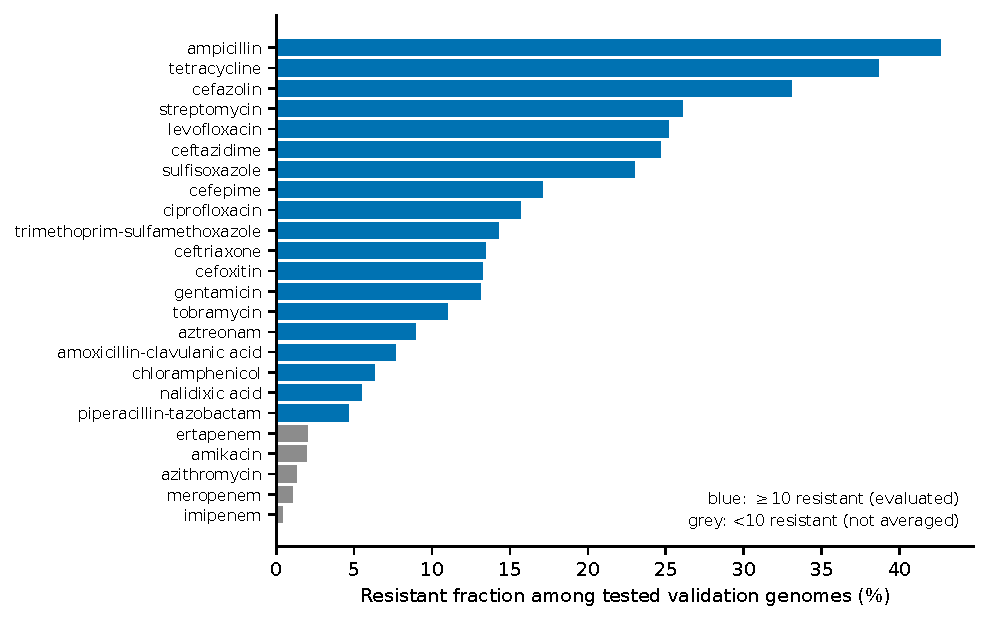
\includegraphics[width=0.78\linewidth]{figures/label_prevalence.pdf}
  \caption{Resistant fraction among tested genomes in the validation split, for antibiotics with at least 100 tested validation genomes.
  Antibiotics with fewer than 10 resistant validation genomes (grey) are shown but excluded from the macro averages.}
  \label{fig:prevalence}
\end{figure}

\subsection{Proteins}
The 6{,}055 labelled genomes contain 29.0 million protein occurrences but only 1.35 million distinct sequences.
An average genome has about 4{,}758 distinct proteins (maximum 5{,}818). 18.8\% of proteins are longer than 512 amino acids.

\subsection{Split}
Genomes are split at random with a fixed seed (42) into 5{,}450 training and 605 validation genomes.
All models use the same split. We discuss in Section~\ref{sec:limits} why a random split is optimistic.

\section{Methods}
\subsection{Protein embeddings}
Each distinct protein sequence is embedded once with \texttt{facebook/esm2\_t12\_35M\_UR50D} \citep{lin2023} in half precision.
Sequences longer than 512 residues are truncated, residue representations are mean-pooled, and the result is a 480-dimensional vector per protein.
Embedding the 1.35 million sequences took about 32 minutes on one NVIDIA A10 GPU.
A genome is then represented by the multiset of the vectors of its proteins; for the sequence heads, also by the order of its proteins in the annotation.
The 1.3\,GB embedding matrix is kept on the GPU during training.

\begin{figure}[t]
  \centering
  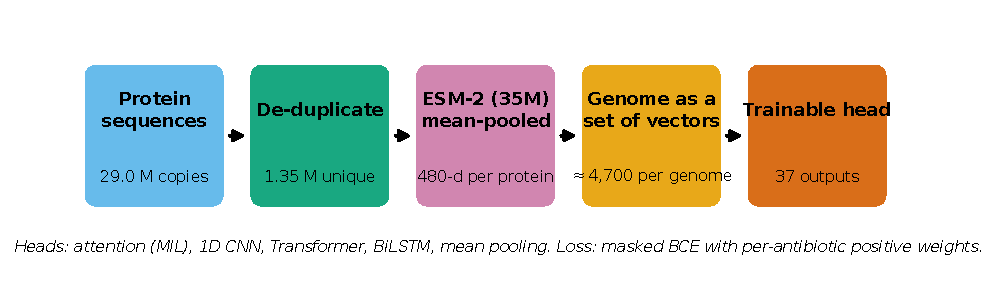
\includegraphics[width=\linewidth]{figures/pipeline.pdf}
  \caption{Overview of the pipeline. Proteins are de-duplicated and embedded once; a trainable head reads all of a genome's embeddings and predicts resistance for 37 antibiotics.}
  \label{fig:pipeline}
\end{figure}

\subsection{Heads}
All heads first apply LayerNorm, a linear layer to 128 dimensions, GELU and dropout (0.2) to each protein vector. They differ in how they aggregate the proteins of a genome.
\begin{description}
  \item[Mean.] Mean over proteins followed by a linear output layer (baseline).
  \item[Attention (MIL).] Gated attention \citep{ilse2018} with a separate attention map for each antibiotic, so different antibiotics can attend to different proteins. During training 20\% of a genome's proteins are hidden at random.
  \item[Transformer.] A 2-layer pre-norm Transformer encoder \citep{vaswani2017} (4 heads, feed-forward width 256) over the set of proteins, followed by mean and max pooling. Trained on random subsets of 1{,}024 proteins per genome and evaluated on all.
  \item[CNN.] Parallel 1D convolutions with kernel sizes 3, 5, 7 and 9 along the genome (in annotation order), followed by mean and max pooling. Trained on random contiguous windows of 1{,}536 proteins.
  \item[BiLSTM.] A single-layer bidirectional LSTM \citep{hochreiter1997} along the genome, then mean and max pooling. Same cropping as the CNN.
\end{description}
At evaluation time all heads read all proteins of a genome.
The Transformer, CNN and BiLSTM heads aggregate with mean and max pooling then a linear layer; the attention and mean heads use a per-antibiotic linear read-out.

\subsection{End-to-end baseline}
As a reference for what happens without precomputed embeddings, we trained a CNN protein encoder end to end on a random sample of 64 proteins per genome (resampled every epoch), with attention pooling over proteins.
It cannot see most of a genome's proteins, and its encoder is trained from scratch rather than pretrained.

\subsection{Training objective and optimisation}
One model predicts all 37 antibiotics. Untested (genome, antibiotic) pairs are masked out of the loss. For each antibiotic $j$ we use a binary cross-entropy with positive weight
$w_j = \mathrm{clip}(N_j^{-}/N_j^{+},\,1,\,10)$, where $N_j^{\pm}$ count resistant/susceptible training genomes.
We use AdamW \citep{loshchilov2019} (learning rate $10^{-3}$, weight decay 0.01), batch size 16 genomes, gradient-norm clipping at 1.0 and up to 30 epochs,
with early stopping (patience 8) on validation macro AUPRC. The BiLSTM head was trained for 10 further epochs at a learning rate of $5\times10^{-4}$ because it was still improving at epoch 30; we report this continued run.
Training times on an A10 GPU for 30 epochs were about 2 minutes (CNN, mean), 3.5 minutes (attention), 10 minutes (Transformer) and 18 minutes (BiLSTM).

\subsection{Evaluation}
We compute the area under the ROC curve (AUROC) and the area under the precision--recall curve (AUPRC) \citep{davis2006} for each antibiotic on its tested validation genomes, and average over
antibiotics with at least 10 resistant validation genomes (21 antibiotics) to obtain macro scores.
AUPRC is reported alongside AUROC because most antibiotics are imbalanced. Antibiotics with fewer resistant genomes are reported but not averaged.

\section{Results}
\subsection{Comparison of heads}
Table~\ref{tab:macro} and Figure~\ref{fig:macro} give macro results. The attention head has the highest macro AUROC (0.931) and the CNN head the highest macro AUPRC (0.798).
The attention, CNN and Transformer heads are within 0.008 AUROC and 0.026 AUPRC of each other; with a single run per head and 605 validation genomes we cannot separate them.
The BiLSTM is somewhat lower (0.912 after continued training; 0.904 at 30 epochs), and mean pooling is clearly lowest among the embedding-based heads (0.843).
The end-to-end baseline reaches 0.593 AUROC and scores below 0.60 for 13 of the 21 antibiotics.

\begin{table}[t]
  \centering
  \caption{Macro-averaged validation performance over the 21 antibiotics with at least 10 resistant validation genomes. Single run per head (seed 42).}
  \label{tab:macro}
  \begin{tabular}{llcc}
    \toprule
    Head & Reads proteins as & AUROC & AUPRC \\
    \midrule
    Attention (gated MIL) & set & 0.931 & 0.786 \\
    1D CNN & ordered sequence & 0.925 & 0.798 \\
    Transformer & set & 0.923 & 0.772 \\
    BiLSTM (+10 epochs) & ordered sequence & 0.912 & 0.753 \\
    Mean pooling & set & 0.843 & 0.621 \\
    \midrule
    End-to-end CNN, 64 proteins/genome & set (sample) & 0.593 & 0.340 \\
    \bottomrule
  \end{tabular}
\end{table}

\begin{figure}[t]
  \centering
  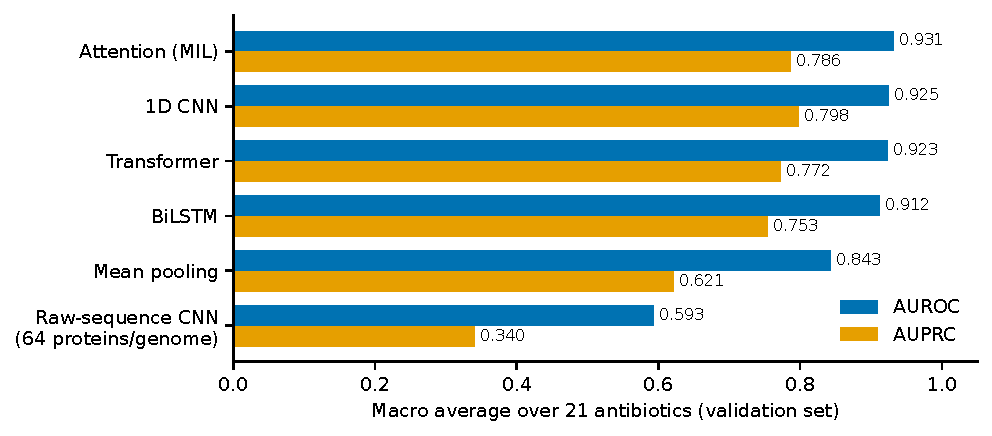
\includegraphics[width=0.85\linewidth]{figures/macro_metrics.pdf}
  \caption{Macro AUROC and AUPRC on the validation split.}
  \label{fig:macro}
\end{figure}

\subsection{Per-antibiotic results}
Table~\ref{tab:per} and Figure~\ref{fig:heat} show AUROC per antibiotic.
Several antibiotics are predicted very well by the better heads (for example aztreonam, cefotaxime, levofloxacin, sulfisoxazole, with AUROC at or above 0.97 for at least one head),
while piperacillin--tazobactam (0.67--0.78 across heads), amoxicillin--clavulanic acid, cefoxitin and ampicillin are harder (best AUROC 0.86--0.88).
Ampicillin is the antibiotic with the most tested genomes yet is not among the best predicted.
Estimates for antibiotics with few tested or few resistant genomes (for example sulfamethoxazole, $n=35$, and cefotaxime, $n=54$ with 51 resistant) are very noisy; the per-antibiotic differences between heads there should not be interpreted.
We did not compute confidence intervals.

\begin{table}[t]
  \centering
  \caption{Per-antibiotic validation AUROC. $n$: tested validation genomes; $n_R$: resistant among them. Best head per row in bold.}
  \label{tab:per}
  \footnotesize
  \begin{tabular}{lrrccccc}
\toprule
Antibiotic & $n$ & $n_R$ & Attention & CNN & Transformer & BiLSTM & Mean \\
\midrule
ampicillin & 584 & 249 & \textbf{0.877} & 0.854 & 0.867 & 0.850 & 0.794 \\
tetracycline & 567 & 219 & \textbf{0.953} & 0.907 & 0.922 & 0.882 & 0.785 \\
ciprofloxacin & 581 & 91 & 0.954 & \textbf{0.966} & 0.935 & 0.959 & 0.870 \\
cefazolin & 248 & 82 & \textbf{0.921} & 0.896 & 0.886 & 0.907 & 0.846 \\
trimethoprim-sulfamethoxazole & 539 & 77 & 0.966 & 0.945 & \textbf{0.968} & 0.936 & 0.904 \\
ceftazidime & 308 & 76 & \textbf{0.973} & 0.963 & 0.939 & 0.960 & 0.875 \\
gentamicin & 573 & 75 & 0.962 & 0.930 & \textbf{0.997} & 0.893 & 0.888 \\
ceftriaxone & 550 & 74 & 0.958 & \textbf{0.976} & 0.955 & 0.959 & 0.823 \\
streptomycin & 276 & 72 & 0.947 & \textbf{0.973} & 0.968 & 0.873 & 0.829 \\
levofloxacin & 266 & 67 & \textbf{0.979} & 0.977 & 0.938 & 0.967 & 0.927 \\
sulfisoxazole & 274 & 63 & 0.983 & 0.982 & \textbf{0.993} & 0.966 & 0.835 \\
cefepime & 304 & 52 & 0.942 & 0.939 & 0.922 & \textbf{0.943} & 0.858 \\
cefotaxime & 54 & 51 & \textbf{0.993} & 0.987 & 0.954 & 0.967 & 0.928 \\
cefoxitin & 371 & 49 & 0.835 & \textbf{0.884} & 0.821 & 0.872 & 0.634 \\
amoxicillin-clavulanic acid & 485 & 37 & 0.831 & 0.852 & 0.790 & \textbf{0.859} & 0.656 \\
tobramycin & 255 & 28 & 0.944 & 0.942 & \textbf{0.982} & 0.938 & 0.917 \\
sulfamethoxazole & 35 & 27 & 0.926 & 0.792 & \textbf{1.000} & 0.792 & 0.866 \\
aztreonam & 223 & 20 & \textbf{0.988} & 0.979 & 0.978 & 0.960 & 0.941 \\
chloramphenicol & 301 & 19 & 0.962 & \textbf{0.963} & 0.962 & 0.935 & 0.930 \\
nalidixic acid & 309 & 17 & 0.921 & 0.959 & 0.949 & \textbf{0.963} & 0.929 \\
piperacillin-tazobactam & 259 & 12 & 0.737 & 0.750 & 0.666 & \textbf{0.777} & 0.662 \\
\midrule
Macro mean & & & 0.931 & 0.925 & 0.923 & 0.912 & 0.843 \\
\bottomrule
\end{tabular}

\end{table}

\begin{figure}[t]
  \centering
  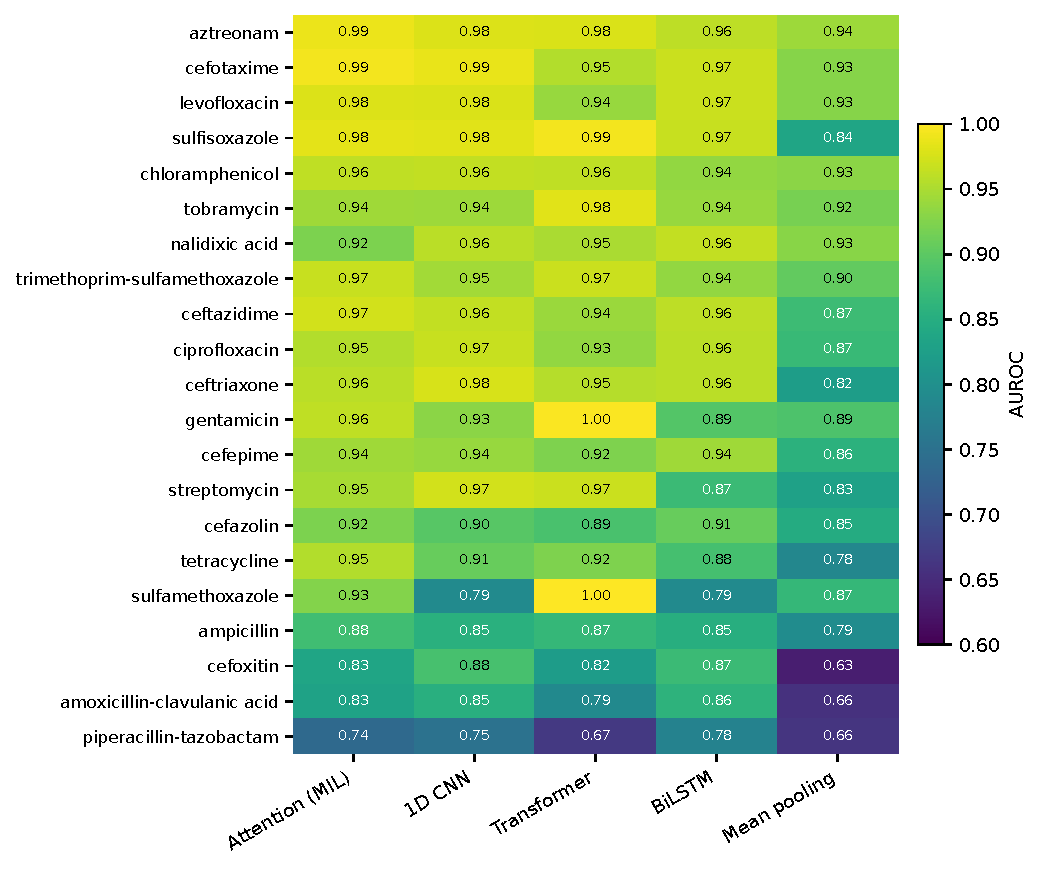
\includegraphics[width=0.75\linewidth]{figures/per_antibiotic_heatmap.pdf}
  \caption{Per-antibiotic validation AUROC for each head, antibiotics sorted by mean AUROC across heads.}
  \label{fig:heat}
\end{figure}

\section{Discussion}
\paragraph{Aggregation matters.}
With identical embeddings, replacing uniform averaging with a learned aggregation lifts macro AUROC from 0.843 to above 0.90 for every other head.
A plausible explanation is that resistance determinants are a tiny fraction of a genome's proteins and a mean over $\approx 4{,}700$ vectors dilutes them.
We have not tested this explanation directly, for example by inspecting attention weights.

\paragraph{Set versus order.}
Heads that use genome order (CNN, BiLSTM) do not clearly outperform heads that treat the genome as a set (attention, Transformer).
Order in these assemblies is partly an artefact of how contigs are arranged, so the absence of an advantage should not be read as evidence that gene neighbourhood is uninformative.

\paragraph{The end-to-end gap is confounded.}
The gap between the end-to-end baseline (0.593) and the embedding-based heads (about 0.92) combines at least three differences: a pretrained versus a from-scratch encoder,
64 sampled proteins versus all proteins, and training cost. We cannot attribute it to any single factor from these experiments.
A controlled ablation (for example the attention head restricted to 64 random proteins) would separate the last two.

\section{Limitations}\label{sec:limits}
These results are preliminary, and we consider the following limitations material.
\begin{enumerate}
  \item \textbf{No independent test set.} The best epoch and early stopping were chosen on the same 605 validation genomes on which we report scores, so reported numbers are mildly optimistic.
  \item \textbf{Random, not lineage-aware, split.} \textit{E.~coli} genomes in public collections cluster into closely related lineages and outbreaks. With a random split, near-identical genomes can appear on both sides, so the model can partly rely on lineage identity. Performance on novel lineages is likely lower.
  \item \textbf{Single seed and no uncertainty estimates.} Differences of about 0.01 between heads are within what we would expect from seed and split variation.
  \item \textbf{No conventional baseline.} We did not run a gene presence/absence or $k$-mer model with logistic regression or gradient boosting, the standard comparison in the AMR literature \citep{moradigaravand2018}. Without it we cannot say how much of the performance requires a neural model or a protein language model.
  \item \textbf{Training length.} The BiLSTM, attention and mean heads were still improving at the 30-epoch limit.
  \item \textbf{Rare antibiotics.} Sixteen of the 37 antibiotics have fewer than 10 resistant validation genomes and are not evaluated, including clinically important carbapenems.
  \item \textbf{Label provenance.} Phenotype labels were produced by different laboratories and methods, and we have not examined label noise.
  \item \textbf{No interpretability analysis.} We do not show which proteins drive predictions or whether they correspond to known resistance determinants.
\end{enumerate}

\section{Conclusion and future work}
Embedding every distinct protein once with a pretrained protein language model makes genome-level resistance prediction on a few thousand \textit{E.~coli} genomes feasible on a single modest GPU,
and heads that learn how to aggregate a genome's proteins perform much better than uniform averaging.
To turn this benchmark into reliable conclusions, the next steps are: (i) a lineage-aware train/validation/test split, (ii) several seeds with confidence intervals, (iii) a gene presence/absence baseline,
(iv) controlled ablations separating encoder pretraining from the number of proteins seen,
(v) attribution analyses checking whether the proteins that drive predictions match known resistance genes, and (vi) larger encoders and additional species from the corpus.

\section*{Data and code availability}
The dataset is publicly available on Hugging Face \citep{bacbench}. Code, trained heads, metrics and logs are available at \url{https://github.com/singam96/bacbench-slm}.
Embeddings can be regenerated with the provided scripts in roughly 30 minutes on a single A10 GPU.

\section*{Acknowledgements}
\todo{Funding, compute and data acknowledgements.}

\begin{thebibliography}{9}
\bibitem[Davis and Goadrich(2006)]{davis2006}
Davis, J. and Goadrich, M. (2006).
The relationship between precision-recall and ROC curves.
In \emph{Proceedings of the 23rd International Conference on Machine Learning (ICML)}.

\bibitem[Hochreiter and Schmidhuber(1997)]{hochreiter1997}
Hochreiter, S. and Schmidhuber, J. (1997).
Long short-term memory.
\emph{Neural Computation}, 9(8):1735--1780.

\bibitem[Ilse et~al.(2018)]{ilse2018}
Ilse, M., Tomczak, J. and Welling, M. (2018).
Attention-based deep multiple instance learning.
In \emph{Proceedings of the 35th International Conference on Machine Learning (ICML)}, PMLR 80:2127--2136.

\bibitem[Lin et~al.(2023)]{lin2023}
Lin, Z., Akin, H., Rao, R., et~al. (2023).
Evolutionary-scale prediction of atomic-level protein structure with a language model.
\emph{Science}, 379(6637):1123--1130.

\bibitem[Loshchilov and Hutter(2019)]{loshchilov2019}
Loshchilov, I. and Hutter, F. (2019).
Decoupled weight decay regularization.
In \emph{International Conference on Learning Representations (ICLR)}.

\bibitem[Moradigaravand et~al.(2018)]{moradigaravand2018}
Moradigaravand, D., Palm, M., Farewell, A., Mustonen, V., Warringer, J. and Parts, L. (2018).
Prediction of antibiotic resistance in \emph{Escherichia coli} from large-scale pan-genome data.
\emph{PLoS Computational Biology}, 14(12):e1006258.

\bibitem[Vaswani et~al.(2017)]{vaswani2017}
Vaswani, A., Shazeer, N., Parmar, N., et~al. (2017).
Attention is all you need.
In \emph{Advances in Neural Information Processing Systems (NeurIPS)}, 30.

\bibitem[BacBench(n.d.)]{bacbench}
BacBench antibiotic-resistance protein sequences dataset.
Hugging Face Datasets, \url{macwiatrak/bacbench-antibiotic-resistance-protein-sequences}.
\todo{verify the authors, title and any associated publication before submission}
\end{thebibliography}

\end{document}
